\chapter{Numerabilidad}%
\label{cha:numerabilidad}

\section{Axiomas}%
\label{sec:axiomas}
\subsection{I Axioma}%
\label{sub:i_axioma}

\begin{defi}[I Ax.]
$X$ es \textbf{1\textsuperscript{er} axioma} si $\forall x \in X,\ \exists \mathcal{V}^x$ base numerable de entornos.  
\end{defi}

\begin{obs}
\begin{enumerate}
    \item $\mathcal{B}^x = \{U_k = \mathring{V}_k \}_{k \ge 1}$, base numerable de entornos de abiertos.
    \item $\mathcal{W}^x = \{W_k = U_1 \cap \ldots \cap U_k\}_{k \ge 1}$, base numerable de entornos abiertos encajados.
    \begin{demo}
        Sea $\left\{ V_k^x, k \ge 1 \right\}$ base de entornos abiertos. Hacemos que: $W_1^x = V_1^x,\ W_2^x = V_1^x \cap V_2^x \ldots W_k^x = \bigcap_{i = 1}^{\infty} V_i^x$ y tenemos que:
        \[
        W_{k+1}^x \subset W_{k}^x
        \]
        que mantiene el ser base de entornos abiertos ($x \in \bigcap_{i = 1}^{\infty} V_i^x$).
    \end{demo}
\end{enumerate}
\end{obs}

\begin{ej}
\begin{enumerate}
    \item $\mathbb{R}^n, \mathcal{T}_u$ cumple el I Axioma
    \begin{demo}    
        Sea $x \in \mathbb{R}^n \Rightarrow \mathcal{W}^x = \{B\left( x, y_k \right): k \ge 1\}$ es base de entornos.
    \end{demo}
    \item $\left( X, \mathcal{T}_a \right), \left( X, \mathcal{T}_{\text{discreta}} \right)$ cumplen el I Axioma.
    \item $\left( \mathbb{R}, \mathcal{T}_{\text{CF}} \right)$ no es I Axioma.
    \begin{demo}
    Veámoslo por reducción al absurdo. Supongamos que $\exists V^x$ numerable $\Rightarrow$

    $\exists \mathcal{W}^x = \{W_k\}_{k \ge 1}$ abiertos encajados, $W_k = \mathbb{R} \setminus F_k$ finito $\Rightarrow \bigcap_{k \in \mathbb{N}} W_k = \mathbb{R} \setminus \bigcup_{k \in \mathbb{N}} F_k \neq \emptyset \Rightarrow \exists y \in \bigcap_{k \in \mathbb{N}} W_k \Rightarrow U^x = \mathbb{R}\setminus \{y\} \not \supset W_k,\ \forall k \in \mathbb{N}$ (porque $y$ pertenece a todos los $W_k$). Por tanto, los $W_k$ no son encajados y tenemos una contradicción. $\left( \bot \right)$
    \end{demo}
\end{enumerate}
\end{ej}

\begin{defi}[Límites]
Decimos que $\lim_{k \rightarrow \infty} x_k = x \Leftrightarrow$ 
\[
\forall U^x,\ \exists k_0 : k \ge k_0 \Rightarrow x_k \in U^x
\]
\end{defi}
\begin{obs}
\begin{enumerate}
    \item $X$ es Hausdorff $\Rightarrow \exists! $ límite. 
    \begin{demo}    
    $x_k \rightarrow x \neq y,\ \exists U^x \cap U^y = \emptyset \Rightarrow \{x_k : k \ge k_0\} \subset U^x$ y $x_k \not \rightarrow y$.
    \end{demo}

    \item El I Axioma permite describir la topología con sucesiones:
    \[
     x \in \overline{A} \Leftrightarrow \exists \{x_k\} \subset A, x_k \rightarrow x
    \]

    \begin{demo}
    \begin{itemize}
        \item[$\Rightarrow)$] Supongamos que $x \in \overline{A} \Rightarrow$
        \[
        \begin{rcases}
            \exists \mathcal{W}^x = \{W_k\}_{k \ge 1} \text{ encajados} \Rightarrow \exists x_k \in W_k \cap A\\
            \forall U^x \stackrel{\text{base ent.}}{\supset} W_{k_0} \supset W_{k + 1} \supset \ldots \Rightarrow x_k \in U^x,\ \forall k \ge k_0  
        \end{rcases} \Rightarrow x_k \rightarrow x
        \]
        \item[$\Leftarrow)$]
        \[
        A \ni x_k \rightarrow x \Rightarrow \forall U^x,\ \exists x_{k_0} \in U^x \cap A
        \]
    \end{itemize}
    \end{demo}
\end{enumerate}
En general, los límites de sucesiones son poco útiles.
\end{obs}

\subsection{II Axioma}%
\label{sub:iiax}
\begin{defi}[II Ax.]
$X$ es \textbf{2º axioma} si $\exists \mathcal{B}$, base numerable de abiertos
\end{defi}

\begin{prop}
\begin{enumerate}
    \item II Ax. $\Rightarrow$ I Ax. 
    \item I Ax $\not \Rightarrow$ II Ax. 
\end{enumerate}
\end{prop}
\begin{demo}
\begin{enumerate}
    \item $\mathcal{B} = \{B_k\}_{k \ge 1} \Rightarrow \mathcal{B}^x = \{B_k : x \in B_k\}$
    \item Espacio discreto no numerable.
\end{enumerate}
\end{demo}

\begin{obs} 
    $\left( \mathbb{R}^n, \mathcal{T}_{u} \right)$ II Ax. $\mathcal{B} = \{B \left( q, \frac{1}{k} : q \in \mathbb{Q}^n, k \ge 1 \right)\}$ [Ejercicio].
\end{obs}

\subsection{Separable}%
\label{sub:separable}
\begin{defi}[Separable]
$X$ es \textbf{separable} si $\exists A$, numerable denso.
\end{defi}
\begin{prop}
\begin{enumerate}
    \item II Ax. $\Rightarrow$ separable. 
    \item I Ax. $+$ separable $\not \Rightarrow$ II Ax. 
    \item I Ax. $\not \Rightarrow$ separable. 
    \item Separable $\not \Rightarrow$ I Ax. 
\end{enumerate}
\end{prop}
\begin{demo}
\begin{enumerate}
    \item $\mathcal{B} = \{B_k\}_{k \ge 1} \Rightarrow A = \{\overbrace{a_k}^{\in B_k}\}_{k \ge 1}$ corta a todo abierto.
    \item $\left( X, \mathcal{T}_a \right), X$ no numerable.
    \item Espacio discreto no numerable.
    \item $\left( \mathbb{R}, \mathcal{T}_{CF} \right) : \overline{\mathbb{Z}} = \mathbb{R}$.
\end{enumerate}
\end{demo}

\subsection{Lindelöf}%
\label{sub:lindelof}
\begin{defi}[Lindelöf]
$X$ es \textbf{Lindelöf} si $\forall X = \bigcup_{i} U_i$ (recubrimiento abierto) $\exists X = \bigcup_{k} U_{i_k}$ (subrecubrimiento numerable). 
\end{defi}

Esta forma débil de compacidad se menciona como complemento. [Ejercicios]

\section{Tabla de comportamiento}%
\label{sec:tabla_de_comportamiento_num}
%TODO: Fix table
\begin{table}[H]
\centering 
\begin{tabular}{| c | c | c | c | c |}
\hline
& Subespacios & Cocientes & Productos & Sumas\\
\hline
    I Ax. & \checkmark & \begin{tabular}{@{}c@{}}$\times$\\ abierto \checkmark \end{tabular} & \checkmark & \checkmark\\
    \hline
    II Ax. & \checkmark & \begin{tabular}{@{}c@{}}$\times$\\ abierto \checkmark \end{tabular} & \checkmark & \checkmark\\
    \hline
    Separable & \begin{tabular}{@{}c@{}}$\times$\\ abierto \checkmark \end{tabular} & $\times$ & \checkmark & \checkmark\\
    \hline
    Lindelöf & \begin{tabular}{@{}c@{}}$\times$\\ abierto \checkmark \end{tabular} & \checkmark & $\times$ & \checkmark\\
    \hline
\end{tabular}
\caption{\textit{Tabla que nos indica como se comportan las propiedades que hemos visto en la anterior sección con las distintas construcciones.}}
\end{table}

%TODO: Agrupar mejor como en el "manuscrito azul".
\begin{itemize}
    \item I Ax. y II Ax. se \underline{heredan} a subespacios intersecando bases.
    \item Separable se hereda a subespacios abiertos intersecando el conjunto denso.
    \item Lindelöf se hereda a subespacios cerrados como la compacidad. No en general: $Y$ no Lindelöf, $X = Y \cup \{w\}$ compacto, $\mathcal{B}^w = \{X \setminus F: F \subset Y\}$ con $F$ finito.
\end{itemize}

\begin{itemize}
    \item $X = \mathbb{R}_u$ I y II Ax's, $Y = \mathbb{R}/\mathbb{Z}$ no es I.
    %TODO: Image
    \begin{center}
        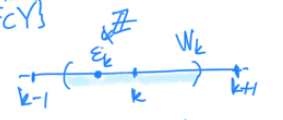
\includegraphics[scale=0.3]{images/ej_axiomas_num_real} 
    \end{center}
    \begin{demo}
        $\alpha = \mathbb{Z} \in Y,\ \exists \mathcal{W}^{\alpha} = \{W_k : k \ge 1\}$ abiertos saturados, $W_k \supset \mathbb{Z},\ \forall k$

        (figura) $\Rightarrow U = \mathbb{R} \setminus \{\varepsilon_k : k \ge 1\}$ entorno abierto saturado de $\mathbb{Z} U \not \supset W_k,\ \forall k$.
    \end{demo}

    \item $\forall$ aplicación continua y abierta conserva I y II 
    \begin{demo}
        Imagen de base es base.
    \end{demo}
    \item $\forall $ aplicación continua conserva separabilidad 
    \begin{demo}
        $f\left( \overline{A} \right) \subset \overline{f\left( A \right)}$.
    \end{demo}
    %TODO: Ya se sabe xd
    \item $\forall$ aplicación continua conserva Lindelöf. 
    \begin{demo}
        Como la compacidad, ya se sabe...
    \end{demo}
\end{itemize}

\begin{itemize}
    \item Para productos: producto finito de numerables es numerable.
    \item Para sumas: suma finita de numerables es numerable.
    \item Solo falla Lindelöf:
    \begin{itemize}
        \item $\left( \mathbb{R}, \mathcal{T}_{[, )} \right)$ es Lindelöf (ejercicio no banal).
        \item $\left( \mathbb{R}^2, \mathcal{T}_{[, )}^2 \right)$ no es Lindelöf: si lo fuera, $L = \{x + y = 0\} \subset \mathbb{R}^2$ heredaría la propiedad, pero es \underline{discreto} no numerable $\bot$.
    \end{itemize}
\end{itemize}
